\documentclass[11pt]{article}
% Language setting
% Replace `english' with e.g. `spanish' to change the document language
\usepackage[spanish]{babel}

% Set page size and margins
% Replace `letterpaper' with`a4paper' for UK/EU standard size
\usepackage[a4paper,top=1.9cm,bottom=2.2cm,left=1.9cm,right=1.32cm,marginparwidth=1.75cm]{geometry}

\setlength{\parindent}{1em}
\setlength{\parskip}{1em}

% Useful packages
\usepackage{amsmath}
\usepackage{mathtools}
\usepackage{graphicx}
\usepackage{xcolor}
% \usepackage{color}% xcolor or color
\usepackage[colorlinks=true, allcolors=blue]{hyperref}

% Set document Font
\usepackage{fontspec}

\setmainfont{Times New Roman}

% Para las ecuaciones: https://latex.codecogs.com/eqneditor/editor.php?lang=es-es

\title{
	Proyecto Global Integrador:
	\\
	Control Semi-Automático Coordinado de Grúa Portuaria de Muelle tipo Pórtico
}

\author{
	Guarise Renzo
	\\
	Trubiano Lucas
	\\
	Profesor: Ing. Gabriel L. Julián
	\\
	\\
	Autómatas y Control Discreto
	\\
	Ingeniería Mecatrónica
	\\
	Universidad Nacional de Cuyo - Facultad de Ingeniería
}

\begin{document}
\maketitle

\begin{center} % Centrar texto
    {\Large \textbf{Resumen}}
\end{center}

Este informe presenta el proyecto de un control semi-automático coordinado de una grúa portuaria de muelle tipo pórtico, desarrollado con Matlab, Simulink y CODESYS. El objetivo del proyecto es diseñar un sistema de control multinivel (Nivel 0, 1 y 2) que permita la coordinación entre las distintas funciones de la grúa, mejorando la eficiencia y seguridad en la carga y descarga de contenedores en el puerto.
\par
Para esto consideraremos unas simplificaciones en el sistema físico; en primer lugar vamos a suponer un movimiento en 2 dimensiones x e y, tanto del contenedor como del carro; consideramos que luego este movimiento se replicaría en cada carril; en segundo lugar para moverse en el plano tendremos en cuenta 2 tipos de movimiento uno de avance/retroceso del carro y otro de izaje del cable, lo que un movimiento de tipo péndulo del contenedor. Dichas simplificaciones sirven para el planteo del modelo matemático y físico de la planta.
\par
Las fases de desarrollo del proyecto se dividen en 2, “Model-in-the-loop” y “Software-in-the-loop”. La primera consta de usar Matlab, Simulink y Stateflow para construir un modelo del sistema y el sistema de control, y realizar pruebas y simulaciones para determinar el correcto funcionamiento de los mismos. Luego la segunda etapa consta de llevar la lógica del autómata a un entorno estandarizado como CODESYS (según norma IEC 61131-3) y realizar una prueba conjunta con comunicación por protocolo OPC UA para verificar el correcto funcionamiento del proyecto.



% \tableofcontents % Creamos el indice
\newpage
\section{Introducción}


Una de las formas más comunes de comercializar y mover productos y/o materias primas en grandes cantidades es a través de contenedores en barcos. Esto se ha difundido de tal forma en el mundo que los puertos son muy comunes y claves para las economías de los países. En estos puertos se mueven grandes cantidades de contenedores, en tiempos muy reducidos para aumentar la eficiencia, y teniendo en cuenta que son objetos pesados hay que manipularlos con una precisión y seguridad que no es fácil de lograr. Para esto se utilizan grúas que son semi-automáticas, es decir, tramos con operación manual y tramos con operación automática. A estas grúas se les dota de sistemas de control lo suficientemente robustos o a prueba de fallas.
\par
Para resolver este problema lo primero es realizar el modelado físico que, por simplificación, consta de un carro en la parte superior que se mueve en dirección horizontal. Y del mismo cuelga  un cable que sostiene el contenedor, este cable se puede izar, de tal forma que, también simplificando el modelo, el sistema queda como el de un carrito con un péndulo de longitud variable. Del extremo del cable cuelga un “spreader” que sostiene el contenedor y esto conforma la carga del péndulo o del cable.
\par
Luego de resolver el modelado físico-matemático del sistema procedemos a desarrollar un autómata que tiene funciones de control y seguridad y está formado por 3 niveles:
\begin{itemize}
    \item \textbf{Nivel 2:} Este controlador está compuesto por otros dos controladores de estados continuos en tiempo discretizado (controles de lazo cerrado), reciben las consignas del controlador superior (Nivel 1) separado por 2 consignas, una de izaje y otra de traslación. Y en base a eso hace un control genérico de 4 cuadrantes sobre los accionamientos electromecánicos. Los controles son PID de movimiento con modulador de torque para izaje y traslación, y control tipo PD para el balanceo.
    \item \textbf{Nivel 1:} Es un controlador de estados discretos que es activado por eventos. Su estructura es jerárquica y concurrente para una mejor performance de las trayectorias. 
    \item \textbf{Nivel 0:} Este nivel es un control también de estados discretos y activado por eventos, que se encarga de detectar condiciones de operación para proteger al sistema y asegurar la confiabilidad del mismo o actuar en casos de fallas y/o colisiones.
\end{itemize}
\par
Estos controladores de los 3 niveles fueron desarrollados primero en Stateflow (componente de Matlab) para facilitar el desarrollo, testeo y simulación de su funcionamiento; ya que este es fácil de integrar con Matlab y Simulink en tiempo real. Así cuando se verificó que estaba bien desarrollado y cumplía con los requerimientos se implementó esa misma lógica en el entorno de desarrollo industrial CODESYS, siguiendo la norma IEC61131.


\newpage


\section{Desarrollo}
Como se mencionó anteriormente, el desarrollo de cualquier proyecto requiere un enfoque sistemático y riguroso, y este proyecto no es una excepción. Para garantizar un resultado exitoso, lo primero que se debe hacer es obtener un \textbf{modelo físico-matemático} preciso y detallado que permita modelar y simular el sistema de la grúa de la forma más exacta posible, teniendo en cuenta las simplificaciones e hipótesis necesarias para hacer el modelo que mejor represente nuestro sistema.
\par
Una vez que se tiene este modelo, es hora de avanzar al siguiente paso crítico: diseñar y optimizar el \textbf{sistema de control}. Este sistema de control es el corazón del proyecto, y se encarga de garantizar que la grúa se mueva con precisión y seguridad en todo momento. Para hacer esto, se deben llevar a cabo simulaciones exhaustivas para identificar y resolver cualquier problema potencial antes de pasar al siguiente paso.
\par
Con el sistema de control diseñado y optimizado, es hora de pasar a la fase de prueba. Aquí, el autómata se convierte en código usando la plataforma de programación \textbf{CODESYS} y se simula el funcionamiento completo del sistema. Se evalúan el rendimiento y la precisión del sistema en condiciones de operación, y se realiza una evaluación rigurosa para garantizar que el sistema cumpla con todas las especificaciones requeridas.
\par
Finalmente, se presentan los \textbf{resultados} obtenidos y las \textbf{conclusiones} finales. Aquí se discuten los logros del proyecto, se identifican las lecciones aprendidas y se destacan los aspectos a mejorar.

\section{Modelado del sistema}

El sistema se compone de dos movimientos fundamentales, el \textbf{sistema de traslación horizontal (carro)}, y el \textbf{sistema movimiento vertical (izaje)}. Vamos a desarrollar las ecuaciones de ambos sistemas por separado y luego veremos cómo esos movimientos se combinan para dar como resultado las ecuaciones de movimiento del contenedor en el \textbf{plano x-y}.

\subsection{Hipotesis}
El sistema planteado es de una complejidad considerable, por lo cuál, para los fines académicos vamos a plantear una serie de simplificaciones o consideraciones sobre el modelo:
\begin{itemize}
	\item Consideraremos la estructura del pórtico como completamente rígida.
	\item El carro que se desliza sobre la estructura, tiene un desplazamiento puramente horizontal y sin resbalamiento.
	\item Los mecanismos de transmisión del carro se consideran rígidos.
	\item Un único cable de acero equivalente de carro siempre tensado (tracción), con elasticidad longitudinal amortiguada.
	\item Asumimos mecanismo equivalente (1 tambor con 1 freno de emergencia, 1 motor con 1 freno) con transmisión rígida.
	\item Un cable de acero equivalente de izaje, con masa propia despreciable, elástico sólo a tracción (no soporta compresión).
	\item Vamos a suponer que no existen efectos externos sobre el carro ni la carga. Es decir, no hay efectos aerodinámicos al chocar con el viento.
	\item El sistema está sometido a la acción de la aceleración de la gravedad, que se aplica verticalmente sobre la carga. Y también a la interacción de contacto o apoyo de la carga o spreader sobre el suelo.
\end{itemize}

\subsection{Sistema de traslación del carro}
Comencemos por el primer sistema de movimiento. Respecto del carro que se mueve en dirección horizontal, debemos tener en cuenta las siguientes especificaciones:
\begin{itemize}
	\item La posición $x_{t}$ varía desde $-30.0\ m$ (en el muelle) hasta $+50.0\ m$ (en el barco).
	\item La velocidad máxima $v_{t}$ es de $4.0\ m/s$ (con o sin carga).
	\item La aceleración máxima $\dot{v_{t}}$ es de $0.8\ m/s^{2}$ (con o sin carga).
\end{itemize}

El carro se mueve sobre los rieles en la parte superior de la grúa en dirección horizontal, eje x, como se muestra en la figura \ref{fig:ref_grua} en donde se esquematizan dichas referencias.

\begin{figure}[h!]
	\centering
	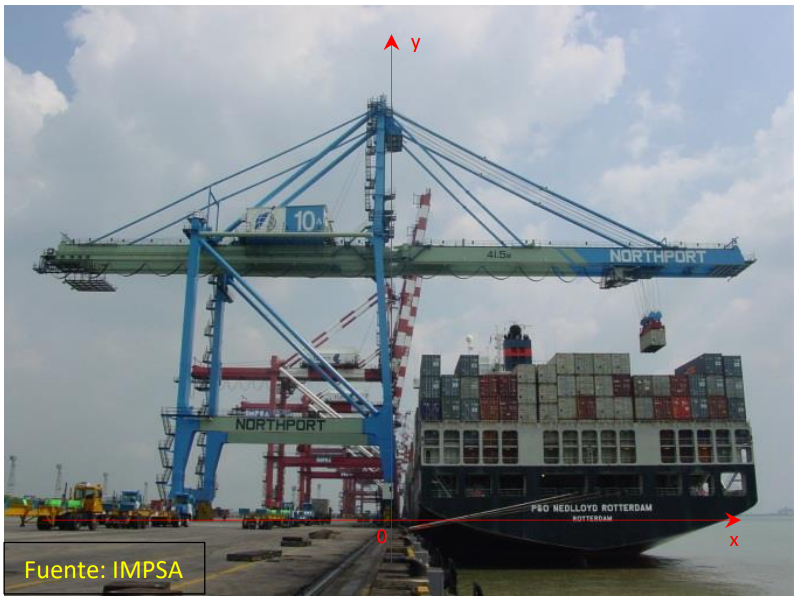
\includegraphics[width=0.85\textwidth]{images/imagen_1_sistema_ref_grua.png}
	\caption{\label{fig:ref_grua} Sistema de referencia de los ejes x e y de la grúa.}
\end{figure}

Luego si analizamos la siguiente figura \ref{fig:sistema_carro} donde se esquematiza el sistema del carro, cable de carro y sistema de transmisión. Podemos ver que el carro se mueve sobre los rieles con un movimiento de rodadura pura (rotación sin deslizamiento), y que el sistema de transmisión del carro se compone de un motor, una caja reductora, un tambor y un freno.

\begin{figure}[h!]
	\centering
	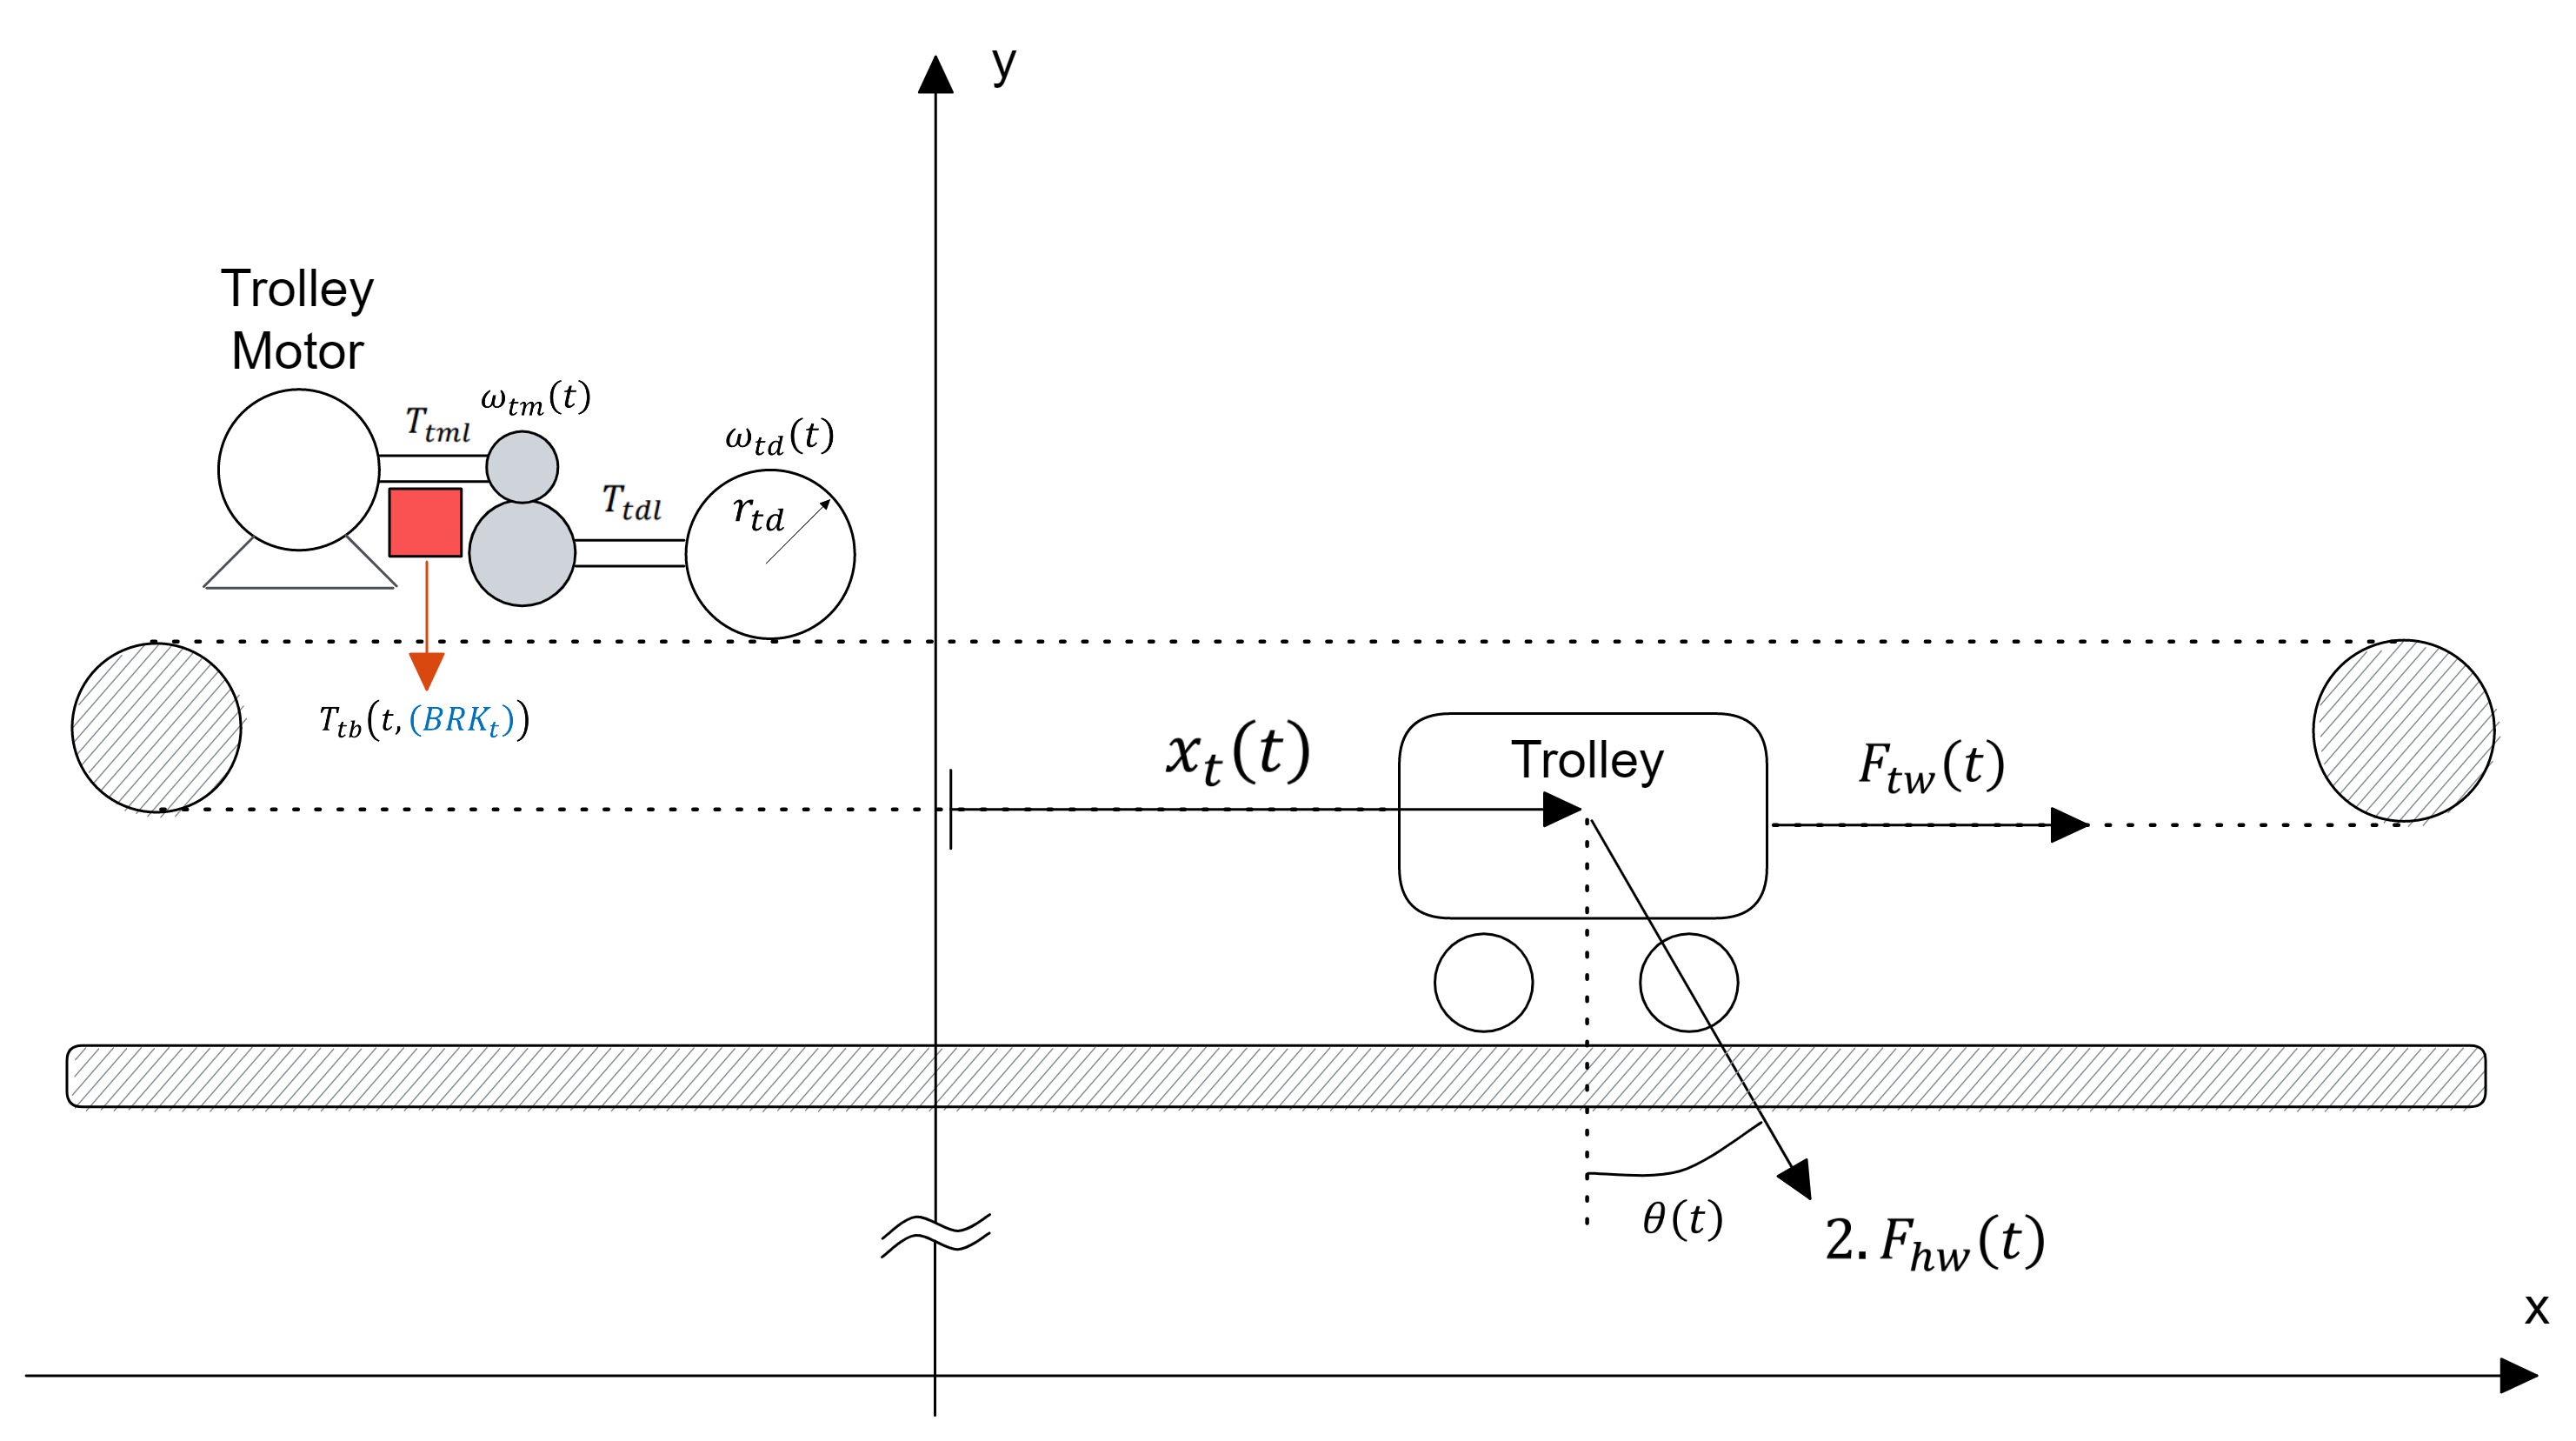
\includegraphics[width=1\textwidth]{images/imagen_2_sistema_carro.png}
	\caption{\label{fig:sistema_carro} Diseño esquemático del sistema del carro.}
\end{figure}
\newpage
A partir de esto podemos deducir la siguiente ecuación \ref{eq:sistema_carro}, que representa el movimiento del carro:
\begin{equation}
	\label{eq:sistema_carro}
	M_{t}\cdot\dot{v}_{t}(t)=F_{tw}(t)-b_{t}\cdot v_{t}(t)+2\cdot F_{hw}(t)\cdot sin(\theta(t))
\end{equation}

Donde:
\begin{itemize}
	\item $M_{t}$ es la masa equivalente del carro, ruedas, etc.
	\item $b_{t}$ es el coeficiente de fricción viscosa equivalente del carro.
	\item $x_{t}$, $v_{t}$ y $\dot{v}_{t}$ son la posición, velocidad y aceleración del carro respectivamente.
	\item $F_{tw}$ es la fuerza de tracción del cable de carro.
	\item $F_{hw}$ es la fuerza que ejerce el cable de izaje sobre el carro (por la acción de la gravedad sobre la carga).
\end{itemize}

Además la fuerza $F_{tw}$ es la que ejerce el cable de carro sobre el carro, y se puede expresar según la ecuación \ref{eq:f_tw}:
\begin{equation}
	\label{eq:f_tw}
	F_{tw}(t)=K_{tw}\left ( x_{td}(t) - x_{t}(t) \right ) + b_{tw}\left ( v_{td}(t) - v_{t}(t) \right )
\end{equation}
Donde:
\begin{itemize}
	\item $K_{tw}$ es la rigidez equivalente total a tracción del cable tensado de carro.
	\item $b_{tw}$ es la fricción interna o amortiguamiento total del cable tensado de carro.
\end{itemize}
Si tenemos en cuenta el radio primitivo del tambor $r_{td}$ y las relaciones $v_{td}(t)=r_{td}\cdot\omega_{td}(t)\ \ ;\ \ F_{tw}(t)\cdot r_{td} = T_{tdl}(t)$. Podemos expresar la ecuación \ref{eq:sistema_carro} referida al eje lento del tambor, como se muestra en la ecuación \ref{eq:sistema_carro_eje_lento}:

\begin{equation}
	\label{eq:sistema_carro_eje_lento}
	J_{td}\cdot \dot{\omega}_{td}(t)=T_{td}(t)-b_{td}\cdot\omega_{td}(t) - T_{tdl}(t)
\end{equation}

Donde:
\begin{itemize}
	\item $J_{td}$ es la inercia equivalente del eje lento (tambor y etapa de salida de la caja reductora).
	\item $b_{td}$ es el coeficiente de fricción viscosa equivalente del eje lento.
	\item $T_{td}$ es el torque de tracción del motor sobre el eje lento (a través de la caja reductora).
	\item $T_{tdl}$ es el torque que ejerce el cable de carro sobre el tambor del eje lento.
\end{itemize}

Y teniendo en cuenta la relación de transmisión entre el motor y el tambor, $i_{t}$, y también las siguientes relaciones $\omega_{td}(t)\cdot i_{t} = \omega_{tm}(t) \ \ ;\ \ T_{td}(t)=i_{t}\cdot T_{tml}(t)$ . Podemos expresar la ecuación \ref{eq:sistema_carro_eje_lento} referida al eje rápido del motor, como se muestra en la ecuación \ref{eq:sistema_carro_eje_rapido}:

\begin{equation}
	\label{eq:sistema_carro_eje_rapido}
	J_{tm+tb}\cdot\dot{\omega}_{tm}(t)=T_{tm}(t)+T_{tb}(t,{\color{blue}BRK_{t}})-b_{tm}\cdot\omega_{tm}(t)-T_{tml}(t)
\end{equation}

Donde:
\begin{itemize}
	\item $J_{tm+tb}$ es el momento de inercia equivalente del eje rápido (motor, disco de freno de operación y etapa de entrada de la caja reductora).
	\item $b_{tm}$ es el coeficiente de fricción viscosa equivalente del eje rápido.
	\item $T_{tb}$ es el torque del freno sobre el eje rápido.
	\item $T_{tm}$ es el torque que ejerce el motor sobre el eje rápido.
	\item $T_{tml}$ es el torque que ejerce la etapa de salida de la transmisión sobre el eje rápido.
\end{itemize}

Si tenemos en cuenta las ecuaciones \ref{eq:sistema_carro}, \ref{eq:sistema_carro_eje_lento} y \ref{eq:sistema_carro_eje_rapido}. Y las reemplazamos y operamos algebraicamente, podemos obtener la ecuación \ref{eq:sistema_carro_final} que representa el movimiento del carro:

\begin{equation}
	\label{eq:sistema_carro_final}
	\begin{matrix}
		M_{t}\cdot\dot{v}_{t}(t)=\frac{T_{tm}(t)\cdot i_{t}}{r_{td}}+\frac{T_{tb}(t,{\color{blue}BRK_{t}})\cdot i_{t}}{r_{td}}-\frac{\left ( b_{td}+b_{tm}\cdot{i_{t}}^{2} \right )}{{r_{td}}^{2}}\cdot v_{td}-\frac{\left ( J_{td}+J_{tm+tb}\cdot{i_{t}}^{2} \right )}{{r_{td}}^{2}}\cdot \dot{v}_{td}\ \ ...
		\\
		\\
		...\ \ -b_{t}\cdot v_{t}+2\cdot F_{hw}(t) \cdot sin \left ( \theta(t) \right )
	\end{matrix}
\end{equation}

En base a la ecuación \ref{eq:sistema_carro_final} el diagrama de bloques en Simulink del modelo del carro queda como se aprecia en la siguiente figura \ref{fig:sistema_carro_simulink}:

\begin{figure}[h!]
	\centering
	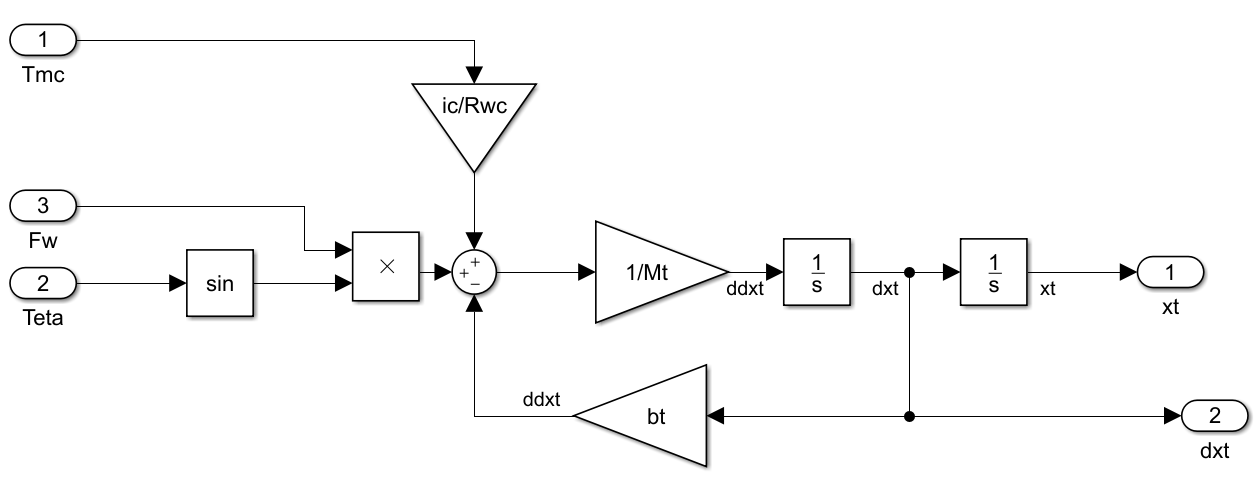
\includegraphics[width=0.8\textwidth]{images/imagen_3_simulink_carro.png}
	\caption{Diagrama de bloques (Simulink) del modelo del carro.}
	\label{fig:sistema_carro_simulink}
\end{figure}

\newpage

\subsection{Sistema de izaje de la carga}

Para el modelado del sistema de izaje tenemos que considerar las limitaciones que detallaremos a continuación:
\begin{itemize}
	\item La posición en $y_{h}\equiv Y_{t0}-l_{h}$ varía desde $-20.0\ m$ (dentro del barco) hasta $+40.0\ m$ (sobre el barco/muelle).
	\item La altura del carro y del sistema de izaje es $Y_{t0}= +45.0\ m$
	\item El despeje mínimo sobre el borde del muelle (sill beam) es $Y_{sb}= +15.0\ m$
	\item Velocidad máxima $v_{h}$: $\pm 1.5\ m/s$ (con carga nominal); $\pm 3.0\ m/s$ (sin carga). Esto es para mantenerse dentro de la curva de potencia constante durante el izaje. Ver figura \ref{fig:curva_potencia_motor}.
	\item Aceleración máxima $\dot{v}_{h}$: $\pm 0.75\ m/s^{2}$ cargado o sin carga.
\end{itemize}

\begin{figure}[h!]
	\centering
	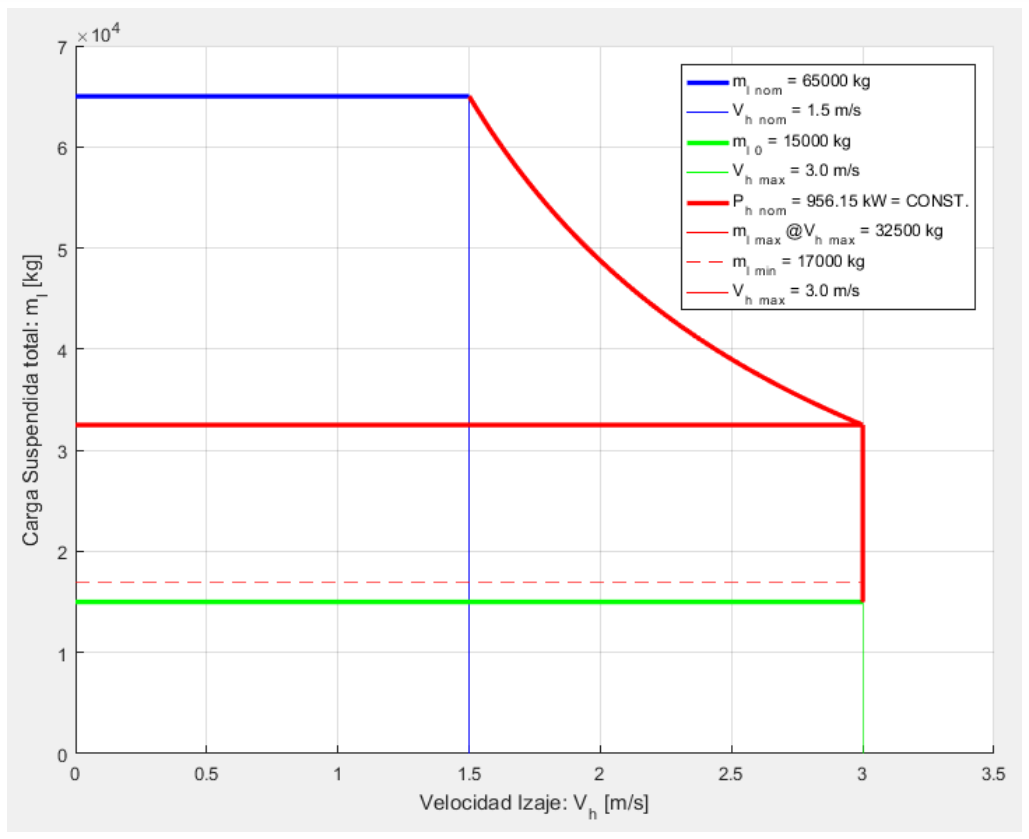
\includegraphics[width=0.7\textwidth]{images/imagen_4_curva_pot_cte.png}
	\caption{Característica de Potencia Constante - Carga suspendida vs. velocidad izaje.}
	\label{fig:curva_potencia_motor}
\end{figure}

\newpage

En base a dichas especificaciones y en la siguiente figura \ref{fig:sistema_izaje} que muestra el modelo físico del sistema de izaje.

\begin{figure}[h!]
	\centering
	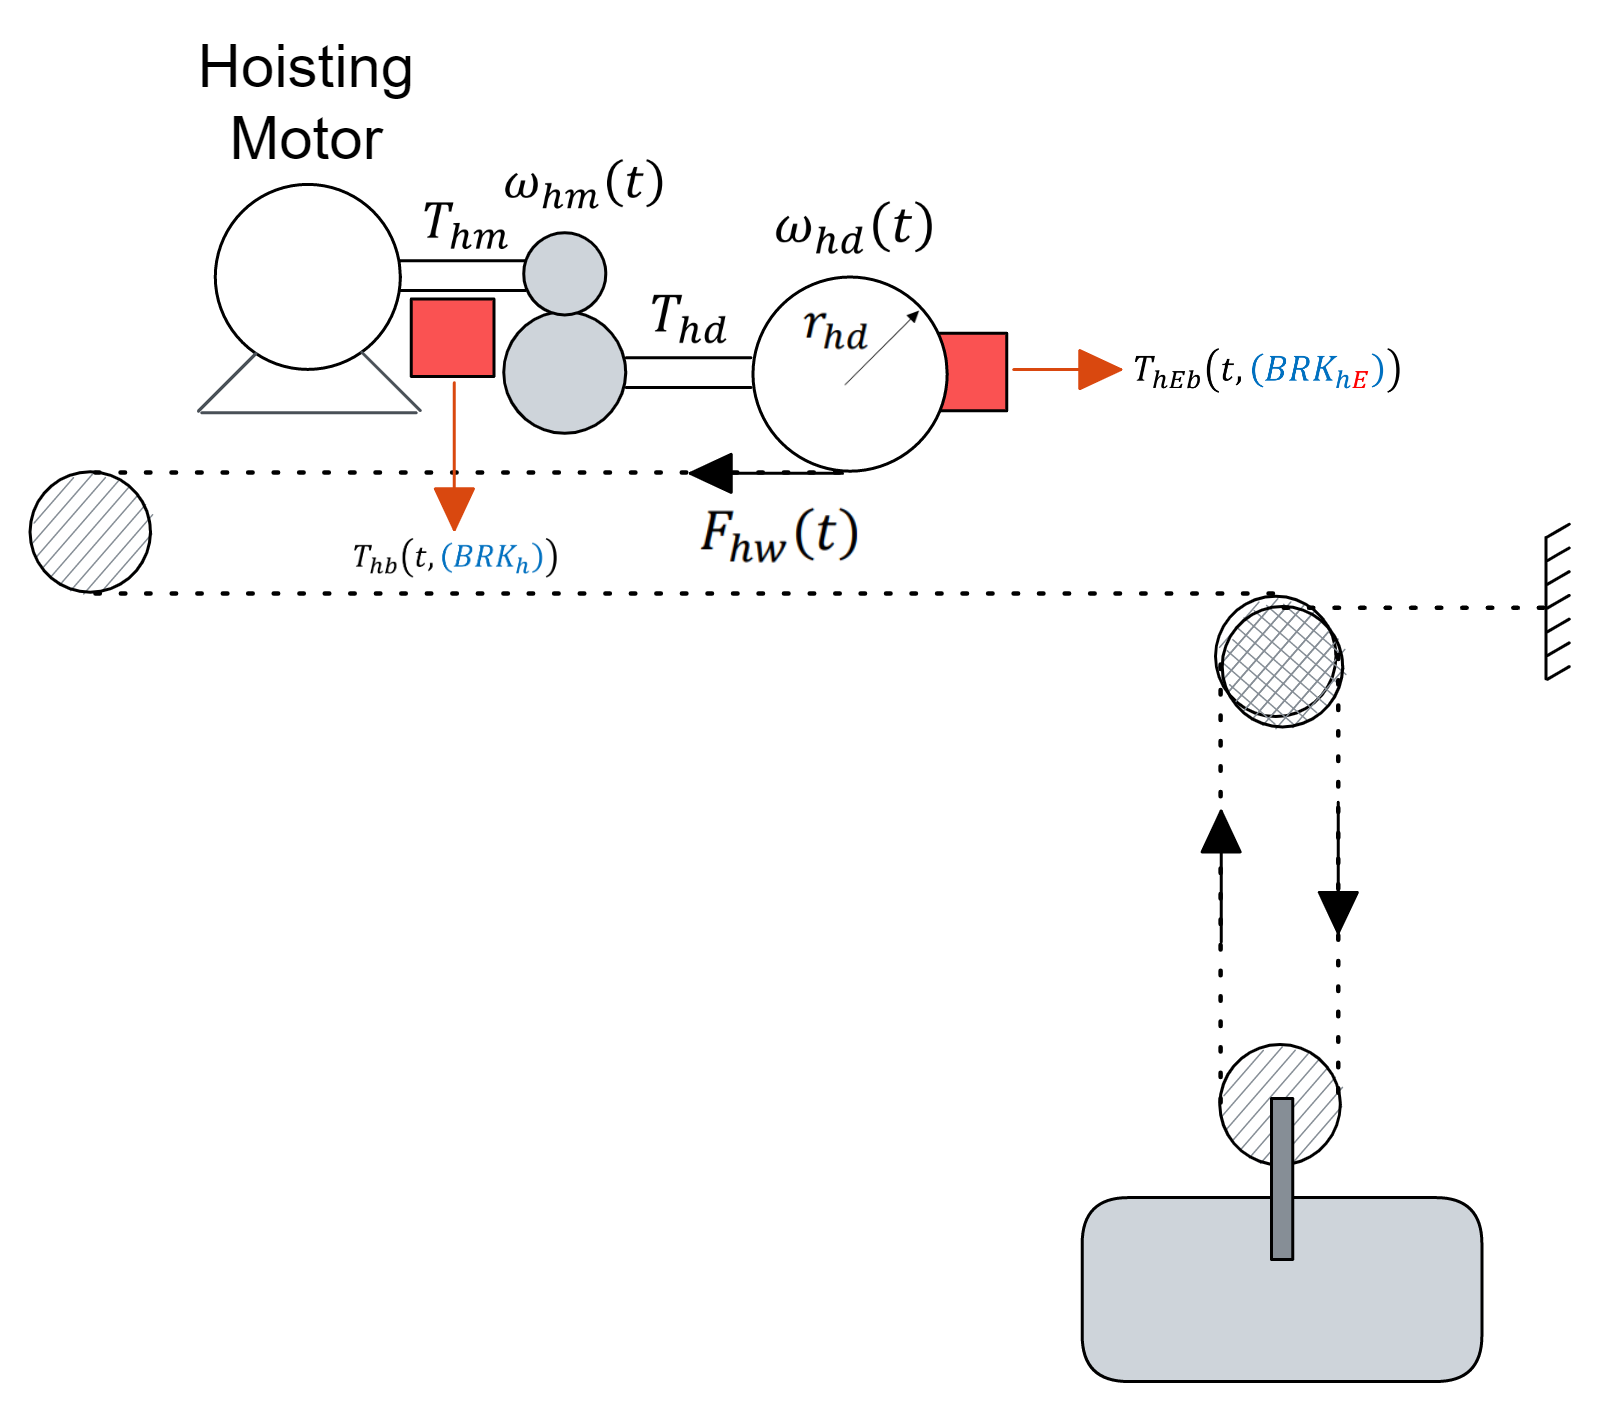
\includegraphics[width=0.85\textwidth]{images/imagen_5_sistema_izaje.png}
	\caption{Diseño esquemático del sistema de izaje y frenos.}
	\label{fig:sistema_izaje}
\end{figure}

Si aplicamos la segunda ley de newton para sistemas rotacionales, se obtiene la siguiente ecuación para el eje del motor (eje rápido):

\begin{equation}
	\label{eq:sistema_izaje_eje_rapido}
	J_{hm+hb}\cdot\dot{\omega}_{hm}(t)=T_{hm}(t)+T_{hb}(t,{\color{blue}BRK_{h}})-b_{hm}\cdot\omega_{hm}(t)-T_{hml}(t)
\end{equation}

Donde:

\begin{itemize}
	\item $J_{hm+hb}$ es el momento de inercia equivalente del eje rápido (motor, disco de freno de operación y etapa de entrada de la caja reductora).
	\item $b_{hm}$ es el coeficiente de fricción viscosa equivalente del eje rápido.
	\item $T_{hm}$ es el torque que ejerce el motor sobre el eje rápido. Torque de motorización o frenado regenerativo.
	\item $T_{hb}$ es el torque que ejerce el disco de freno de operación sobre el eje rápido.
	\item $T_{hml}$ es el torque que ejerce la etapa de salida de la transmisión y las cargas referidas al eje rápido.
\end{itemize}

De forma equivalente, podemos plantear el modelo referido al eje del tambor (eje lento). Teniendo en cuenta que $i_{h}$ es la relación de reducción entre el eje rápido y el eje lento, podemos decir que $\omega_{hd}\cdot i_{h}=\omega_{hm}$ y que $T_{hd}=i_{h}\cdot T_{hml}$.
Así obtenemos la siguiente ecuación \ref{eq:sistema_izaje_eje_lento}:

\begin{equation}
	\label{eq:sistema_izaje_eje_lento}
	J_{hd+hEb}\cdot\dot{\omega}_{hd}(t)=T_{hd}(t)+T_{hEb}(t,{\color{blue}BRK_{hE}})-b_{hd}\cdot\omega_{hd}(t)-T_{hdl}(t)
\end{equation}

Donde:

\begin{itemize}
	\item $J_{hd+hEb}$ es el momento de inercia equivalente del eje lento (tambor, disco de freno de emergencia y etapa de salida de la caja reductora).
	\item $b_{hd}$ es el coeficiente de fricción viscosa equivalente del eje lento.
	\item $T_{hd}$ es el torque que mueve el tambor, referido al eje lento.
	\item $T_{hEb}$ es el torque que ejerce el disco de freno de emergencia sobre el eje lento.
	\item $T_{hdl}$ es el torque de carga referido al eje lento.
\end{itemize}

Además considerando la siguiente ecuación \ref{eq:sistema_izaje_lh} que relaciona la posición ideal que tendría el extremo $x_{h}(t)$ en función de la longitud de cable desenrollada $l_{h}(t)$:

\begin{equation}
	\label{eq:sistema_izaje_lh}
	Y_{t0}-l_{h}(t)\equiv x_{h}(t) \Rightarrow -\dot{l_{h}}(t)=\dot{x}_{h}(t)\equiv v_{h}(t)
\end{equation}

Y si además tenemos en cuenta el radio primitivo del tambor de izaje $r_{hd}$, podemos decir que:

\begin{equation}
	\label{eq:sistema_izaje_vh}
	2\cdot v_{h}(t)=r_{hd}\cdot \omega_{hd}(t)\ \ \ ;\ \ \ F_{hw}(t)\cdot r_{hd}=T_{hdl}(t)
\end{equation}

Si operamos algebraicamente con las ecuaciones \ref{eq:sistema_izaje_eje_rapido}, \ref{eq:sistema_izaje_eje_lento}, \ref{eq:sistema_izaje_lh} y \ref{eq:sistema_izaje_vh}. Reemplazando y acomodando términos podemos llegar a la siguiente ecuación \ref{eq:sistema_izaje_final}:

\begin{equation}
	\label{eq:sistema_izaje_final}
	\begin{matrix}
		2\left ( \frac{{i_{h}}^{2}J_{hm+hb}+J_{hd+hEb}}{{r_{hd}}^{2}} \right )\dot{v}_{h}=\frac{i_{h}\left ( T_{hm}(t)+T_{hb}(t,{\color{blue}BRK_{h}}) \right )+T_{hEb}(t,{\color{blue}BRK_{hE}})}{r_{hd}}\ \ ...
		\\
		\\
		...\ \ -2\left ( \frac{{i_{h}}^{2}b_{hm}+b_{hd}}{{r_{hd}}^{2}} \right )v_{h}-F_{hw}
	\end{matrix}
\end{equation}

Notemos que la ecuación \ref{eq:sistema_izaje_final} está en función de la posición $x_{h}(t)$, la velocidad $v_{h}(t)$ y la aceleración $\dot{v}_{h}(t)$ del extremo ideal (si no estuviera estirado el cable). Por lo tanto, la fuerza que experimenta el cable, que tiene en cuenta la longitud de cable desenrollada y la longitud real del cable (consecuencia del estiramiento) tiene la siguiente ecuación \ref{eq:sistema_izaje_fuerza_cable}:

\begin{equation}
	\label{eq:sistema_izaje_fuerza_cable}
	\left\{
		\begin{matrix*}[l]
		F_{hw}(t)=2\cdot K_{w}\left ( l_{h}(t) \right )\cdot \left ( l(t)-l_{h}(t) \right )+2\cdot b_{w}\left ( l_{h}(t) \right )\cdot ( \dot{l}(t)-\dot{l_{h}}(t) ) \ \ \Leftrightarrow\ \ l(t)\geq l_{h}(t)
		\\
		\\ 
		F_{hw}(t)= 0\ \ \Leftrightarrow\ \ l(t)<l_{h}(t)
		\end{matrix*}
	\right.
\end{equation}

Donde:

\begin{equation}
	\label{eq:sistema_izaje_fuerza_cable_params}
	K_{w}\left ( l_{h}(t) \right )=\frac{K_{wu}}{2\cdot l_{h}(t)+110\ m}\ \ \ ;\ \ \ b_{w}\left ( l_{h}(t) \right )=b_{wu}\cdot \left ( 2\cdot l_{h}(t)+110\ m \right )
\end{equation}

\section{Análisis de tipos de carga}
\subsection{Análisis con carga suspendida}
\subsection{Análisis con carga apoyada}

\section{Sistemas de control}
\subsection{Nivel 2 - Controladores de movimiento}
\subsubsection{Controlador de posición del carro}
\subsubsection{Controlador del izaje de la carga}
\subsubsection{Controlador del péndulo (ángulo de balanceo de la carga)}
\subsection{Nivel 1 - Control supervisor}
\subsection{Nivel 0 - Control de seguridad}

\section{Simulación}
\section{Implementación en CODESYS}
\section{Pruebas finales. Servidor OPC UA.}
\section{Resultados}
\section{Conclusiones}
\section{Referencias}










\newpage
FIN DOCUMENTO
\newpage


% ejemplo de espacio entre párrafos
% \vspace{0.3cm}\\

% ejemplo de letras minúsculas enumeradas
% \renewcommand{\theenumi}{\alph{enumi}} %Letras minúsculas

% ejemplo de imagen
% \begin{figure}[h!]
% 	\centering
% 	\includegraphics[width=\textwidth]{2_1_2_ModeloElectricoEquivalente.png}
% 	\caption{\label{fig:ElectricoEquivalente} Diagrama en bloques de la planta completa en \textbf{Simulink} (con transformación de \textbf{Park})}
% \end{figure}


\section{Referencias}

[1] Apuntes de cátedra. Automática y Maquinas Eléctricas. Profesor Ing. Gabriel Julián.

[2] Ingeniería de Control Moderna, 5ta edición, Katsuhiko Ogata, 2010.

[3] Analysis of Electric Machinery and Drive Systems, 3° Ed. Krause, P. et al.

[4] Guía del Proyecto Global Integrador. Automática y Maquinas Eléctricas. Profesor Ing. Gabriel Julián

\end{document}